% 2 side format
\documentclass[epsfig,a4paper,11pt,titlepage,twoside,openany]{book}
\usepackage{epsfig}
\usepackage{plain}
\usepackage{setspace}
\usepackage{graphicx}
\usepackage{listings}
\usepackage{float}
\usepackage{multirow}
\usepackage[paperheight=29.7cm,paperwidth=21cm,outer=1.5cm,inner=2.5cm,top=2cm,bottom=2cm]{geometry} % layout setting
\usepackage{titlesec} % custom setup title of chanpter
% \usepackage{newtxtext,newtxmath} % times new roman

%%%%%%%%%%%%%%
% support for accented letters
%
%\usepackage[latin1]{inputenc} % Windows;
\usepackage[utf8x]{inputenc} % Linux (unicode package is required);
%\usepackage[applemac]{inputenc} % Mac.

\singlespacing

%code personalization
\usepackage{listings}
\usepackage{xcolor}

\definecolor{codegreen}{rgb}{0,0.6,0}
\definecolor{codegray}{rgb}{0.5,0.5,0.5}
\definecolor{codepurple}{rgb}{0.58,0,0.82}
\definecolor{backcolour}{rgb}{0.95,0.95,0.92}

\lstdefinestyle{mystyle}{
    backgroundcolor=\color{backcolour},   
    commentstyle=\color{codegreen},
    keywordstyle=\color{magenta},
    numberstyle=\tiny\color{codegray},
    stringstyle=\color{codepurple},
    moredelim=**[is][\color{magenta}]{@}{@},
    moredelim=**[is][\color{codegreen}]{~}{~},
    basicstyle=\ttfamily\footnotesize,
    breakatwhitespace=false,         
    breaklines=true,                 
    captionpos=b,                    
    keepspaces=true,                 
    numbers=left,                    
    numbersep=5pt,                  
    showspaces=false,                
    showstringspaces=false,
    showtabs=false,                  
    tabsize=2
}

\lstset{style=mystyle}

\begin{document}

  % no page number
  \pagenumbering{gobble} 
  \pagestyle{plain}

\thispagestyle{empty}

\begin{center}
  \begin{figure}[h!]
    \centerline{
\psfig{file=marchio_unitrento_colore_it_202002.eps,width=0.6\textwidth}}
  \end{figure}

  \vspace{2 cm} 

  \LARGE{Department of Information Engineering and Computer Science\\}

  \vspace{1 cm} 
  \Large{Bachelor's Degree in Computer Science}

  \vspace{2 cm} 
  \Large\textsc{Final Dissertation\\} 
  \vspace{1 cm} 
  \Huge\textsc{Validation and flexibility evaluation of a new ROS2-BDI architecture}
  %\Large{\it{Sub-title (optional)}}


  \vspace{2 cm} 
  \begin{tabular*}{\textwidth}{ c @{\extracolsep{\fill}} c @{\extracolsep{\fill}} c }
  \Large{Advisor} & \Large{Coadvisors} & \Large{Student}\\
  \Large{Paolo Giorgini} & \Large{Marco Robol} & \Large{Redi Vreto}\\
  \Large{}& \Large{Marco Roveri} & \Large{}\\
  \Large{}& \Large{} & \Large{}\\
  \end{tabular*}

  \vspace{2 cm} 

  \Large{Academic year 2022/2023}
  
\end{center}



  \clearpage

  \thispagestyle{empty}

\begin{center}
  {\bf \Huge Acknowledgements}
\end{center}

\vspace{4cm}

\emph{
 thanks to
}

\vspace{3cm}

\emph{Professor Giorgini for giving me the opportunity to carry out this project}

\vspace{3cm}

\emph{Professors Marco Roveri and Marco Robol for all the assistance and and advice provided}

\vspace{3cm}

\emph{Devis for all the support when debugging}

\vspace{3cm}

\emph{My family for their love and support}

\vspace{3cm}

\emph{My friends who always manage to put a smile on my face even after long sessions at the library}
  \clearpage
  \pagestyle{plain} % no heading, footer with centered page number

  
  % page number with Arabic format
  \mainmatter

%%%%%%%%%%%%%%%%%%%%%%%%%%%%%%%%%%%%%%%%%%%%%%%%%%%%%%%%%%%%%%%%%%%%%%%%%%
%%%%%%%%%%%%%%%%%%%%%%%%%%%%%%%%%%%%%%%%%%%%%%%%%%%%%%%%%%%%%%%%%%%%%%%%%%
%% Note
%%%%%%%%%%%%%%%%%%%%%%%%%%%%%%%%%%%%%%%%%%%%%%%%%%%%%%%%%%%%%%%%%%%%%%%%%%
%% The maximum number of pages is 30, including:
%%   index
%%   abstract
%%   chapters
%% Excluding:
%%   frontispiece
%%   acknowledgements 
%%   attachments
%%
%% For further details and updated rules, please check the guidelines.
%%%%%%%%%%%%%%%%%%%%%%%%%%%%%%%%%%%%%%%%%%%%%%%%%%%%%%%%%%%%%%%%%%%%%%%%%%
%%%%%%%%%%%%%%%%%%%%%%%%%%%%%%%%%%%%%%%%%%%%%%%%%%%%%%%%%%%%%%%%%%%%%%%%%%

    % index
    \tableofcontents
    \clearpage
    
    
          
    % group to define space between chapters
    \begingroup
      % no page break between chapters
      % override clear page commands
      \renewcommand{\cleardoublepage}{} 
      \renewcommand{\clearpage}{} 
      % override format of title chapter
      % from
      %   Chapter X
      %   Title
      % to
      %   X   Title
      
      \titleformat{\chapter}
        {\normalfont\Huge\bfseries}{\thechapter}{1em}{}
        
      \titlespacing*{\chapter}{0pt}{0.59in}{0.02in}
      \titlespacing*{\section}{0pt}{0.20in}{0.02in}
      \titlespacing*{\subsection}{0pt}{0.10in}{0.02in}
      
      % summary / abstract
      %\chapter*{Abstract} % no number
\label{abtract}

\addcontentsline{toc}{chapter}{Abstract} % add to index

Lorem ipsum dolor sit amet, consectetur adipiscing elit. Donec sed nunc orci. Aliquam nec nisl vitae sapien pulvinar dictum quis non urna. Suspendisse at dui a erat aliquam vestibulum. Quisque ultrices pellentesque pellentesque. Pellentesque egestas quam sed blandit tempus. Sed congue nec risus posuere euismod. Maecenas ut lacus id mauris sagittis egestas a eu dui. Class aptent taciti sociosqu ad litora torquent per conubia nostra, per inceptos himenaeos. Pellentesque at ultrices tellus. Ut eu purus eget sem iaculis ultricies sed non lorem. Curabitur gravida dui eget ex vestibulum venenatis. Phasellus gravida tellus velit, non eleifend justo lobortis eget.






%%%%%%%%%%%%%%%%%%%%%%%%%%%%%%%%%%%%%%%%%%%%%%%%%%%%%%%%%%%%%%%%%%%%%%%%%%
%%%%%%%%%%%%%%%%%%%%%%%%%%%%%%%%%%%%%%%%%%%%%%%%%%%%%%%%%%%%%%%%%%%%%%%%%%
%% Note
%%%%%%%%%%%%%%%%%%%%%%%%%%%%%%%%%%%%%%%%%%%%%%%%%%%%%%%%%%%%%%%%%%%%%%%%%%
%% The abstract is a short summary of the work describing the target,
%% the subject of the thesis, the methodology and the techniques,
%% the data collection and elaboration, the explanation of the
%% reached results and the conclusion.
%% The abstract of the dissertation must have a maximum length of 3 pages
%% and must include the following information:
%%   context and motivation
%%   short summary of the main problem you have dealt with
%%   developed and /or used techniques 
%%   reached results, the personal contribution of the student has to be highlighted
%%%%%%%%%%%%%%%%%%%%%%%%%%%%%%%%%%%%%%%%%%%%%%%%%%%%%%%%%%%%%%%%%%%%%%%%%%
%%%%%%%%%%%%%%%%%%%%%%%%%%%%%%%%%%%%%%%%%%%%%%%%%%%%%%%%%%%%%%%%%%%%%%%%%%      
      
      %%%%%%%%%%%%%%%%%%%%%%%%%%%%%%%%
      % chapters
      %
      % \input or \include
      %
      \chapter{Introduction}
\section{Context and motivation}
A team of researchers at the University of Trento developed a new general purpose BDI-based robotic system with ROS2. In synthesis this new framework allows programmers to automatically plan and execute actions which fulfill desires following the BDI (belief, desire, intention) philosophy, all whilst using the solid ROS2 communication techniques in the background. 
\par
For instance if one wanted to use this framework to automate robots which retrieve objects inside of a warehouse, all they would need to do is specify what the world looks like using a PDDL domain (what this is specifically will be explained later on); which actions can be performed and their definition (again, the particulars of this will be clear further on). The only thing that is left is to use ROS2 communication tools to continually update the framework on the state of the world.  
\par
The ROS2-BDI framework comes in two flavors: the offline version and the online version. Oversimplifying, the offline approach computes a plan and executes it until failure or success, rescheduling if and only if a failure occurs. The online version on the other hand initiates the execution as soon as it has plan, even if incomplete, then, during execution, if it observes any problems/opportunities it recomputes the plan with the goal of yielding a better solution. For instance, if the agent's goal is to pick up trash and it notices that there is some additional trash to pick up, it will try to come up with a plan to do just that.
\par
The framework is brand new, so much so that a solid validation has not yet been performed. Some attempts at it have been carried out by its creators, however, they do not always make use of industrially recognized tools such as Webots. A simulation was implemented using an ad hoc environment, which may not always be representative of a real world scenario. Conversely, Webots, which is a 3D graphical robot simulator, allows to have a better view of what a real world implementation could look like. 
\section{Problem overview}
In light of all this the first part of the project's objective was dual: firstly, it would try to demonstrate the effectiveness of the framework on Webots; secondly, it tries to show that in highly dynamic environments the online approach bests the offline system. This was accomplished by creating multiple situations where the goal can be quantifiable and hence maximized.
\par
The second part of the project was dedicated to studying the flexibility of the framework. In other words it was tried to prove that once the initial setup is completed, it is pretty straightforward to modify or update the code to fulfill the new objective. This was done by analyzing the differences in code when different kind of changes to the environment or objective were made.
\section{Accomplished results}
The most noteworthy accomplishment is the set of simulations that were created, which not only serve the purpose to validate the efficacy of the ROS2-BDI robotic system, but also as a reference for future researchers/developers who will have the pleasure to work with the framework. The code was written following widely known software engineering guidelines at the best of the abilities of the author, hopefully that makes the code readable and easy to follow as an implementation example. To clarify, what is trying to be said is that the code could be consulted to have a good idea of how to interface with the framework and how to use it in real world scenarios. 


      \chapter{Basic Notions}
\section{ROS2}
ROS2, which stands for robot operating system, is a set of tools and libraries used in robotics applications. Its main objective is to provide an easy and functional way of communicating between processes, which in a real world scenario would each be connected to a functional part of the robot performing some sort of action and interface with other parts when and if necessary. The standard communication principle is the subscribe topic technique.
\subsection{Nodes}
Nodes are the core concept of ROS2, they are each represented by a traditional process and can subscribe and/or publish to topics and services and provide or utilize actions. In a real world example they would logically represent some part of a robot, or a single robot altogether. The ROS2 communication library allows nodes to communicate with each other. The default languages used to define the node's behavior are \texttt{C++} and \texttt{Python3}. Interestingly, it does not matter whether we use one language or the other. ROS2 allows the developer to define the behavior of a node in \texttt{C++} and another in \texttt{Python3} and still have them communicate with each other appropriately.
\subsection{Packages}
Packages contain multiple nodes inside of them. When running a node we must always specify its package. In addition to the nodes behavior specification one can define a launcher which runs multiple nodes following any logic the user may want to follow; a \texttt{XML} and \texttt{CMAKE} file which take care of dependencies and last but not least custom messages, services or actions if one wishes to use them. Although it is a widely followed convention to specify custom interfaces in a separate package.
\subsection{Topics}
Topics are the most used communication tool across nodes in ROS2. They are so fundamental that they could be the only tool used to communicate, even in substitution of actions and services. They are unidirectional and have a many to many relationship, in other words multiple nodes can publish to a single topic and multiple nodes can read the same message at their earliest convenience. A topic is identified using its id, which is used by the publisher to identify in which topic to publish and to the subscriber to decide from which topic to read a message from. The messages sent are used defined based on primitive programming data types such as \texttt{int}, \texttt{char}, \texttt{bool}, etc... Or can also be created including other user defined messages which at their core are primitive data types.   
\subsection{Services}
Services are used whenever a client server architecture is needed, therefore, unlike topics, they are not unidirectional. Here the message does not simply consist of a message containing primitive data types but rather a request message and a response message. As the reader may have already imagined, both the request and response message are user defined messages consisting of primitive data types. One example where one would need services rather than topics would be if we wanted to have one node tell another to do something and to make sure that that action was actually done, which is possible thanks to the response message.
\subsection{Actions}
Actions are very similar to services with the only difference being that they can be interrupted. In addition actions provide multiple response messages during the execution. This allows the issuer to know what percentage of the action has been completed. Like services actions are not essential, for they can be emulated using topics.
\cite{ros2_docs}
\cite{ros2_website}
\section{PDDL}
PDDL stands for planning domain definition language. Like its name suggests it allows the user to define what the world looks like and to feed this definition to a planner which in turn will, whenever possible, output a solution to a problem.
Let us analyze the two main parts of a PDDL problem definition with respect to the 2.1 version, which is the one used by ROS2-BDI.
\subsection{Domain definition}
As anticipated, the domain definition allows the user to define what the world looks like. 
\begin{itemize}
    \item Firstly the \textbf{types} need to be defined. They indicate what kind of object resided in our world. 
    \item \textbf{Predicates} basically are statement about the world which could either be true or false. If a predicate's value is undefined PDDL follows the closed world assumption and assumes everything to be false unless specifically stated otherwise.
    \item \textbf{Actions} indicate which kind of actions can be performed in our world. They are defined by their parameters, which specify the instances in our world which are affected or depend by this action. The duration, which is optional and used only for durative actions, is the time it takes to complete the action. The condition identifies the predicates that must be true for the action to be executed. All conditions must be satisfied at the same time for the action to be considered executable. A condition can be considered \emph{at start}, which means that it needs to be true before the execution even starts; \emph{over all} which means that the condition must be true throughout the execution window and \emph{at end} which is not used in the condition but rather in the effect, which means that the condition will be set to true at the very end of the execution.
    \item \textbf{Effect} states which conditions will be se to true or false at the end (or start if we use the keyword) of the action.
    \item \textbf{Functions} are predicates with real values associated to them. For instance if we wanted to state that the battery of a robot is at 50\% we could say \texttt{battery robot 50}. Needless to say these values can be assigned at the end of an action and can be checked before the execution of one. For example if we wanted to make sure that the robot has enough battery (say 50 \%) at the beginning of the action we could say \texttt{at start (> battery ?robot) 50}. It is also possible to assign a new value to a function or to increase/decrease the current value with a similar syntax.
\end{itemize} 
\subsection{Problem definition} The problem definition's purpose is to define a problem, this is accomplished by:
\begin{itemize}
    \item Detailing which domain this particular problem is referring to.
    \item Listing each object in our world. For instance one could declare the fact that the object whose name shall be \texttt{g} is of type \texttt{robot} by typing \texttt{g - robot}.
    \item Itemizing each true statement at the very beginning of the execution of the world. For example if one wanted to say that the robot \texttt{g} is located at the room \texttt{r} all they would need to write is \texttt{(at g r)}. That is assuming that a predicate \texttt{at} has been previously defined in the domain.
    \item Initialize every function by assigning it a real value.
    \item Specifying the goal. As common sense suggest that is just a list of predicates that we want to be true at the end of the execution of the plan.
\end{itemize}
By doing all of this preliminary work we will be rewarded when we feed our plan to a planner such as Plansys2 because we will be provided with a working plan which has been computed efficiently and automatically.
\cite{pddl_docs}
\section{Webots}
Webots is a 3D robot simulator which is capable of connecting to ROS2 after a little bit of setup. There are countless functionalities which can be used but only the ones that have been used for this project will be described. 
\subsection{World definition} Webots allows its users to define a custom world simply by creating a \texttt{.wbt} file. The idea behind this file is very simple: every object is defined by a reference to a PROTO and the specification of some fields such as the translation (where to position the object), the scale (how much bigger/smaller than default we want this object to be), the color and many many more. A PROTO is a predefined model which specifies every little detail of an object, down to the geometry, physics, contact properties ecc... 
\par
Luckily it gets even easier than that, the user can take advantage of the user interface to create objects and position/modify them as they please. The \texttt{.wbt} file will be modified accordingly and automatically.
\subsection{Robot controller}
Every robot, in addition to initial position and many other properties, has a \texttt{controller} field. This permits the user to define the behavior of the moving parts of the robot, such as the motors. The controller can be defined inside of webots and not use ROS2 communication. Alternatively it can be defined as \texttt{extern} and be controlled by a ROS2 node.
\subsection{Supervisor}
The supervisor is, at its core, a common robot. However, it is capable of much more than a mere robot! In fact it can do whatever it wants. For example it can move objects completely disregarding the physics of the simulation; it can add or remove new objects which can be very helpful for some simulations; it can keep track of the simulation time by reading the \texttt{clock} topic. Being a robot it has a controller, which can very conveniently be a ROS2 node.
\cite{webots_docs}
\section{ROS2-BDI}
As anticipated in the introduction the ROS2-BDI framework comes in two flavors: the offline version and the online version. Their difference is not limited to the way they operate but down to the architectural level. If we wanted to be more precise we should say that there are three versions: the offline version with Plansys2 and the modified version of JAVAFF and the online version with the extension to JAVAFF. Only the first and the latter will be described in the following pages as they were the one used to create the project.
\subsection{Offline ROS2-BDI}
As a reminder, the objective of this design is to have a multi agent framework leveraging all the ROS2 tools and libraries, all while following a BDI based philosophy. Furthermore an automatic planner, Plansys2 in this case, is used to automatically create and execute plans.  

Firstly we shall briefly introduce the architecture of Plansys2 and finally the ROS2-BDI framework built upon it will be presented. 
\subsubsection{Plansys2} Plansys2 is an application whose goal is to compute and execute plans automatically following the PDDL syntax. In short it is able to output a valid plan and to execute it given a pddl domain and a pddl problem.
\par
Since it is built on top of ROS2 its core functionalities are implemented using ROS2 nodes. These core nodes are the executor, the planner, the domain expert and the problem expert. Let us briefly explore these nodes purpose's and interconnections.
\begin{itemize}
    \item The \textbf{executor}, as the name suggests, executes the plan received from the planner. It is connected to each action executor of the client application. Whenever the plan dictates it, it sends an action message to the correspondent client action executor. Furthermore, the executor can be used to modify and cancel the plan via specific ROS2 messages.
    \item The \textbf{planner} communicates via ROS2 services with the domain expert and the problem expert. Basically it looks at the PDDL domain it gets from the domain expert and the PDDL problem it gets from the problem expert and tries to come up with a plan using efficient and reliable algorithms.
    \item The \textbf{domain expert} is basically just a node which forwards the PDDL domain to the planner and gets it from the client application. Unfortunately the domain will always remain the same as Plansys2 does not allow any tempering of it during the execution.
    \item The \textbf{problem expert} is very similar to the domain expert in the sense that it is a node containing the current PDDL problem. However, contrary to the domain it does provide API calls which allow to modify the predicates and functions or to modify/add/cancel the current goal. 
\end{itemize}
\cite{plansys2_docs}
\subsubsection{Architecture} Here is the proposed ROS2-BDI architecture, taken from the official paper.
\begin{figure}[H]
\centering
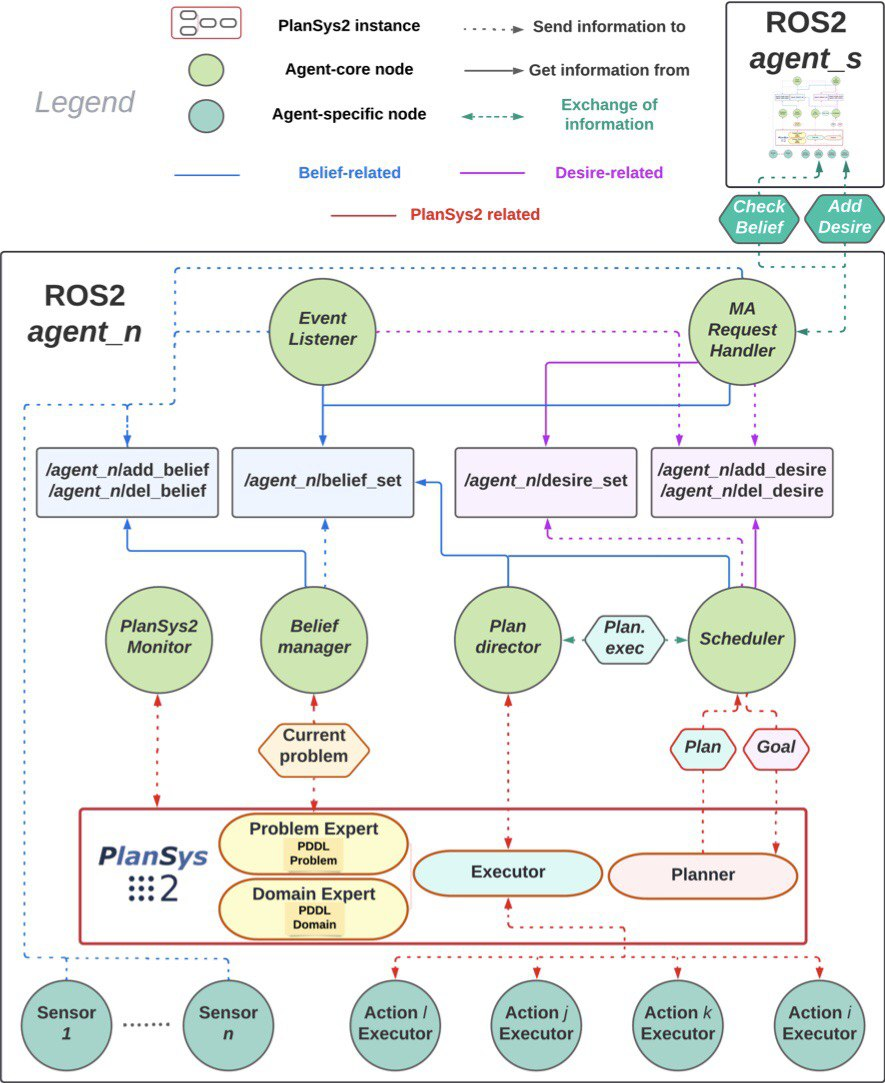
\includegraphics[scale=0.4]{images/offline_architecture.jpg}
\caption{The proposed ROS2-BDI, taken from the official paper}
\end{figure}
It is important to note that all the circles are ROS2 nodes while the rectangles are ROS2 topics. The nodes contained inside the red rectangle compose the Plansys2 instance, every running agent will have its own Plansys2 instance
\par
Let us now shortly go through all the different components that form the ROS2-BDI framework. But before that it is key to differentiate between the different type of nodes in the figure. All the light blue nodes are client application specific and will be different from scenario to scenario. As already mentioned, The red rectangle is the Plansys2 instance and the green nodes are the core nodes of the ROS2-BDI architecture. Everything else is a set of topics with the objective to make the different parts communicate with each other.
\begin{itemize}
    \item \textbf{Plansys2}'s main body is exactly the same way it was described before. It is connected to the client's application action executors and communicates with the core nodes.
    \item The \textbf{sensors} basically look at what is going on in the world and send messages to the topics \texttt{agent\_id/add\_belief} and \texttt{agent\_id/del\_belief} whenever a change occurs. For instance we could have a sensor controlling whether a waypoint is accessible or not. Each and every time the conditions change (i.e. the waypoints switches its state from inaccessible to accessible or vice versa) a message is sent indicating that the belief that the waypoint is accessible needs to be removed or added. It is important to note that the concept of belief is strongly correlated to that of a predicate or function. In fact the belief that the waypoint is accessible is the same as saying that the predicate which indicates that it is is true.
    \item The action executors, like the sensors, are client application dependent. They just wait for an action message to trigger their execution.
    \item The \textbf{Plansys2 monitor}, like its name suggests, continuously exchanges information via ROS2 services with the Plansys2 module to make sure that everything is in working order.
    \item The \textbf{belief manager} has a very basic job, that is to handle request of insertion and deletion of beliefs and to perpetually publish the current beliefs to the \texttt{agent\_id/belief\_set} in order to always have a valid reference. Furthermore, it communicates with the problem expert to make sure that the predicates and functions of the PDDL problem are always up to date. This is an important step that cannot be skipped as the syntax to express a belief differs from that to express a predicate or function.
    \item The \textbf{plan director} basically handles the execution of the plan by initiating it and aborting it if and when necessary.
    \item The \textbf{scheduler} performs a similar job to the belief manager, with the only difference being that it manages the desire set rather than the belief set. In addition to that it decides which plan received from the Plansys2 module to execute and when to abort it or consider it done. 
    \item The \textbf{Event listener} allows to dynamically alter the current state of the world based on the information it receives from the sensors and some rules defined by the programmer. These predefined rules are called reactive rules. For example if we had a world in which the objective is to pick up trash we could, using the reactive rules and the services offered by the request handler, push the desire to retrieve the litter automatically. Obviously these processes are very handy when dealing with dynamic environments where condition change repeatedly.
    \item the \textbf{Multi agent request handler} just forwards the requests from addition and deletion of beliefs and desires.
\end{itemize}
How to practically put ROS2-BDI to use will be clearer in later chapters, for the time being it is enough to have a general idea of how it works.
\cite{ros2_bdi_offline_article}
\cite{ros2_bdi_docs}
\cite{devis_thesis}
\cite{ros2_bdi_offline_demonstration}
\subsection{Online ROS2-BDI} The online version has a lot of similarities to the offline counterpart, both when it comes to the general idea and down to the implementation and means of utilization. 
\par
The main difference in behavior is that the newer online approach start executing a plan even if it is partially created and never stops rescheduling in case new opportunities to fulfill additional desires or to terminate  the execution earlier arise.
\par 
The implementation of the new framework is quite similar in the general structure since it is built upon the offline version as an extension to it. The main differences are the mechanisms which allow to effectuate the new properties and in the planner itself. The planner of choice is a modified version of JAVAFF which has been named OJFF. 
\par 
Since it is possible to switch from the offline version to the online version just by changing some parameters in the launch file the architecture will not be presented as it is extremely similar from a practical point of view.
\subsubsection{OJFF} OJFF is a PDDL 2.1 compliant planner built on top of the JAVAFF planner which allows to follow the properties presented above. The main difference lies in the way the search for a solution is conducted. 
\par
Traditional solution finding algorithms such as the one used by Plansys2 uninterruptedly expand on the search space by adding valid actions at the end of it, all this whilst following well known searching algorithms such as A* and heuristics. This is repeated until exhaustion of the search space or a solution is found. 
\par
On the other hand, OJFF uses another algorithm which differs in the way the search is expanded (it stretches the search from the previous search node until a condition, such as goal reached or maximum depth increment, is met). On top of that it returns the most promising partial solution at the end of each iteration.
\subsubsection{Additional properties needed to make use of temporal planning} Naturally one of these properties is the modified searching algorithm already presented that looks for a solution.
\par
In addition to that a way to forecast the failure of the plan, to improve the solution whenever possible and to revise the goal are necessary. In essence \emph{plan failure forecasting} consists in continually simulating the current plan to check whether it is going to fail or not. In case it does indeed fail, a new plan search which starts from the last committed state is activated. The framework also implements \emph{goal revision} which is the property that allows the planner to try to merge two or more desires in a unique plan whenever possible and more convenient than fulfilling the desires sequentially. Last but not least it adopts a \emph{solution improvement} mechanism which basically means that it tries to make the solution shorter in terms of time whenever possible. That may happen quite often as the framework uses two different algorithm to find a simulation simultaneously. One is quick but usually finds long solutions while the other is slow (with regard to the time it takes to output a valid plan that is) but finds better solutions.
\cite{alex_thesis}
\cite{javaff_repo}
\cite{ojff_repo}
\newpage

      \chapter{Simulation environment}
\label{cap:3}In this chapter the endeavor at a more solid validation in terms of the robustness of the simulator will be presented. Firstly, the setup on the simulator will be introduced. Secondly, the necessary setup correlated to the ROS2-BDI framework will be shown. Finally, the overall architecture will be summarized.
\section{Main scenario description}
Three different scenarios were implemented, only the first shall be explained thoroughly as it is the most basic one. The idea is that there is a $7$  by $7$ grid where objects to continue to appear. The robot's goal is to retrieve these objects and to transfer them to a designated place, the bin. Boxes are placed randomly in the arena with the objective to make the robot's life a little harder.
\begin{figure}[H]
\centering
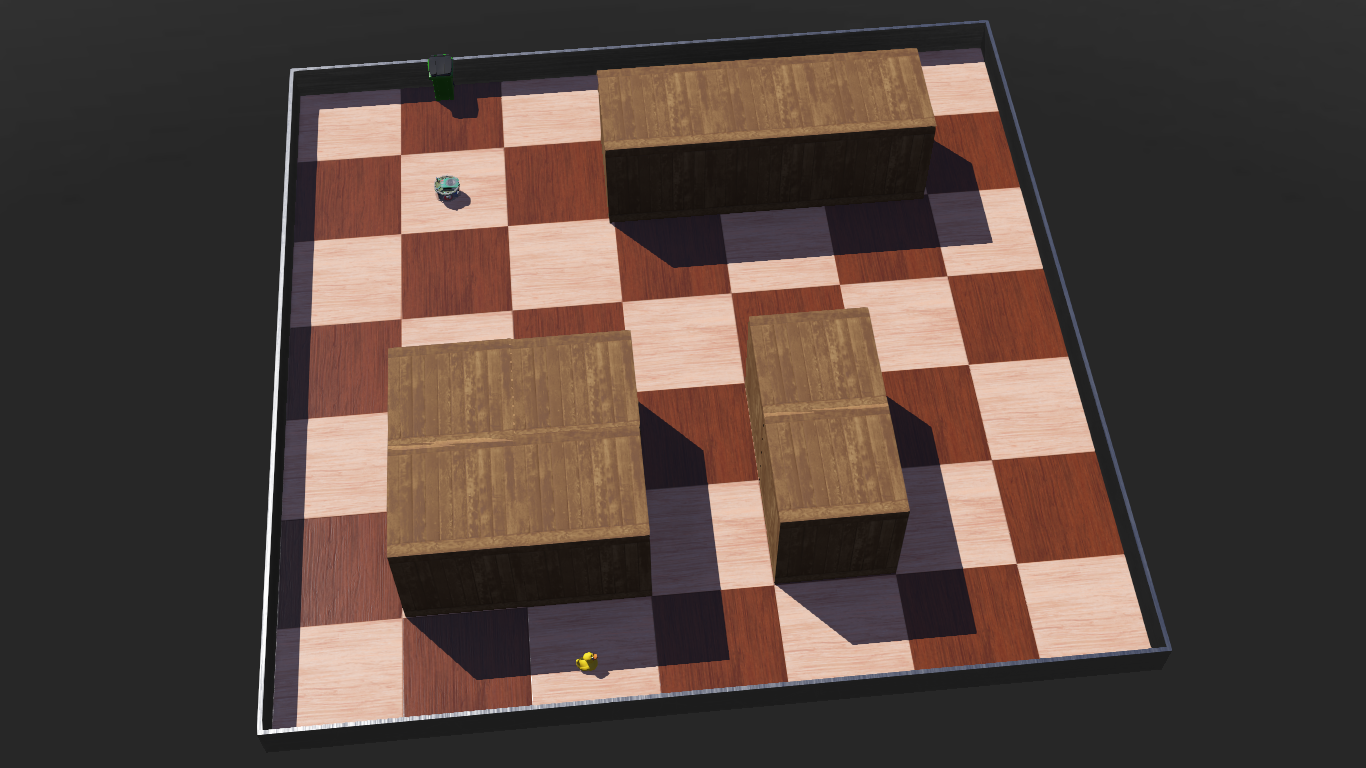
\includegraphics[width=\textwidth]{images/simulation_screen.png}
\caption{Webots simulation in the initial state}
\end{figure}
\section{Webots setup} Let us now look at the necessary steps to take in order to connect the Webots simulator to ROS2, hence enabling it to work with ROS2-BDI.
\par
To begin with, we create a ROS2 package defaulting the node's language to \texttt{Python3} and adding the \texttt{rclpy} library dependency. The original idea was to use \texttt{C++} in order to make the project as consistent as possible with the rest of the implementation, however, the author is not aware of a method which employs the \texttt{C++} language as the official documentation only presents how to use \texttt{Python3}.
\par
A \texttt{setup.py} file needs to be created where all the different resources are declared. These are the world itself, the different robots and the launcher.
\par
Under the \texttt{worlds} directory we need to put the \texttt{.wbt} file which describes what the Webots world looks like.
\par
Inside the \texttt{resources} directory the robot controllers and the supervisor declaration needs to be specified. Here's what the declaration of the main robot looks like: 
\begin{lstlisting}[language=XML, caption=XML file linking robot controller to Webots]
<?xml version="1.0" ?>
<robot name="e_puck">
    <webots>
        <plugin type="spawn_spazza.e_puck_controller.MyRobotDriver" 
        webots_robot_name="e_puck"/>
    </webots>
</robot>
\end{lstlisting}
In line four and five we are specifying the current package \texttt{spawn\_spazza}, the name of the \texttt{Python3} file containing the controller of the robot (\texttt{e\_puck\_controller}) and the name of the class which extends the package needed to create a ROS2 node and which defines the behavior of the robot \texttt{MyRobotDriver}. \texttt{webots\_robot\_name} is used to indicate which robot we are talking about in the simulation.
\par
Now the last step is writing the launcher which is just a file booting up multiple ROS2 nodes. What it does is it enumerates each node to execute, alongside their optional parameters. For example here's what the code launching the robot look like
\begin{lstlisting}[language=Python, caption=launch description for a Webots robot]
        robot_description = pathlib.Path(os.path.join(package_dir, 'resource', 'e_puck.urdf')).read_text()

        my_robot_driver = Node(
        package='webots_ros2_driver',
        executable='driver',
        output='screen',
        additional_env={'WEBOTS_CONTROLLER_URL': controller_url_prefix() + 'e_puck'},
        parameters=[
            {'robot_description': robot_description},
        ],  

        arguments=[
            '--webots-robot-name', 'e_puck',
            '--webots-node-name', 'e_puck'
        ]
    )
\end{lstlisting}
The only thing that is happening here is that we are launching a node whose code is specified inside the \texttt{e\_puck.urdf} file as show above in listing 3.1.
\par
That is all there is to it in the Webots side. Next the implementation of the robot's controller and the supervisor will be discussed.
\section{Robot controller}
\subsection{e\_puck}
The chosen robot was the e\_puck as it is uncomplicated to use and the provided API's are reliable, well documented and work across different languages. 
\par
The e\_puck is a circular robot with seven sensors surrounding it and two wheels on opposite sides controlled by two different motors which can either go forwards or backwards. In order to move forwards it is sufficient to set the speed of both motors to the same positive value. To move backwards the value would need to be negative. Rotating the robot is quite simple as well, we just need to set the speed of the right motor to a positive real value $s$ and $-s$ to the left if we want to rotate anticlockwise. $-s$ and $s$ to rotate clockwise.
\subsection{e\_puck movement mechanisms} Let us now analyze how the movement of the robot works. The e\_puck is placed inside a 3D world with a coordinate system and initially occupies the $(0.0,0.0,0.0)$ position. At some point in the simulation it will receive the order to move to a certain position $(x,y,z)$. The basic idea is to rotate the robot until it faces the target position. Then, move it forwards until it reaches the objective. Here is the pseudocode that shows exactly how this works.
\begin{lstlisting}[language=Python, caption=e\_puck robot movement algorithm]
LEFT = 1, RIGHT = -1
FORWARDS = 1, BACKWARDS = -1
ERROR = 0.01 #error that one is willing to tolerate

def move_robot (robot, pos):
    target_theta = target_theta(robot, pos)
    direction = direction(robot, pos)

    while (abs(robot.theta - target_theta) > ERROR):
        rotate_robot(direction)
    
    while (dist(robot, pos) > ERROR):
        move_robot(FORWARDS)
\end{lstlisting}
\texttt{LEFT}, \texttt{RIGHT}, \texttt{FORWARDS} and \texttt{BACKWARDS} are all constants defined in order to make the code cleaner. While \texttt{ERROR} serves as a way of allowing a small degree of imperfection. 
\par
The implementation of the \texttt{target\_theta} and \texttt{direction} functions are just as fascinating. Let us go over their logic. Before that though we must go through the convention adopted by Webots for the orientation. In the first and second quadrants the angle is defined the same way as it is in mathematics: it starts from $0$ radians and increments all the way to $\pi$ at the end of the second quadrant. The moment it crosses the second quadrant and goes into the third the angle goes from $+\pi$ to $-\pi$, after that it decreases all the way to $0$. Here is a picture to better explain the convention.
\begin{figure}[H]
\centering
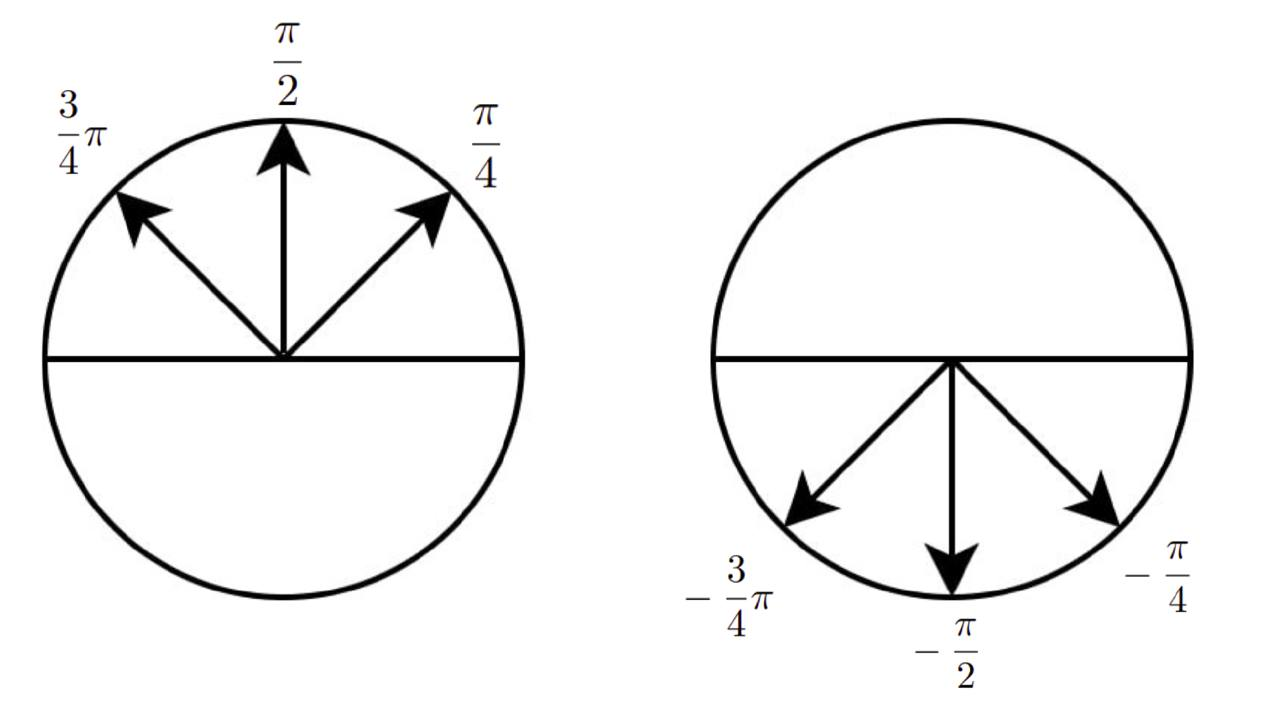
\includegraphics[scale=0.2]{images/webots_angles.jpg}
\caption{Webots orientation convention}
\end{figure}
To rotate the robot towards the objective we start by calculating $\Delta y$ and $\Delta x$ which are respectively the difference in the $y$ and $x$ coordinates between the target and the robot. Under normal circumstances the angle between the robot and the target is defined as $\arctan (\frac{\Delta y}{\Delta x})$. That is because we know from trigonometry that the tangent of $\theta$ is equal to the ratio between the opposite and adjacent side.
\cite{analisi1}
\par
Depending on the sign of $\Delta x$ and $\Delta y$ we split in to four cases:
\newpage
\textbf{$\Delta y > 0 \quad and \quad \Delta x > 0$}: \\ 
\begin{minipage}{0.4\textwidth}
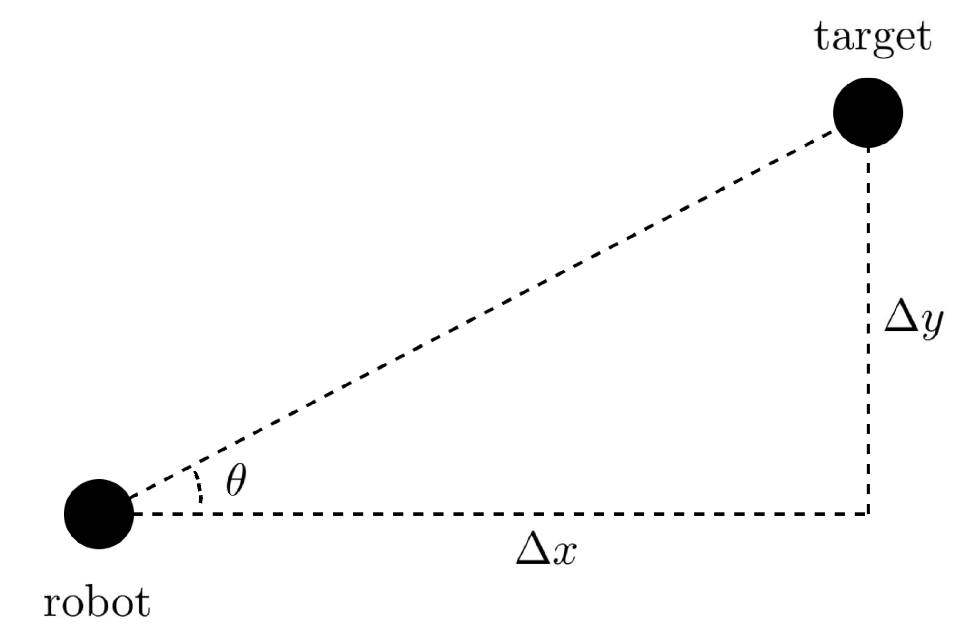
\includegraphics[width=\linewidth]{images/theta1.jpg}
\end{minipage}
\begin{minipage}{0.5\textwidth}\raggedleft
$$\quad \quad \quad \quad \theta = \arctan\left(\frac{\Delta y}{\Delta x}\right)$$ \\
\end{minipage}
\noindent
\\
In this case we simply take the angle between the robot and the target.
\\
\\
\textbf{$\Delta y > 0 \quad and \quad \Delta x < 0$}: \\ \\
\begin{minipage}{0.4\textwidth}
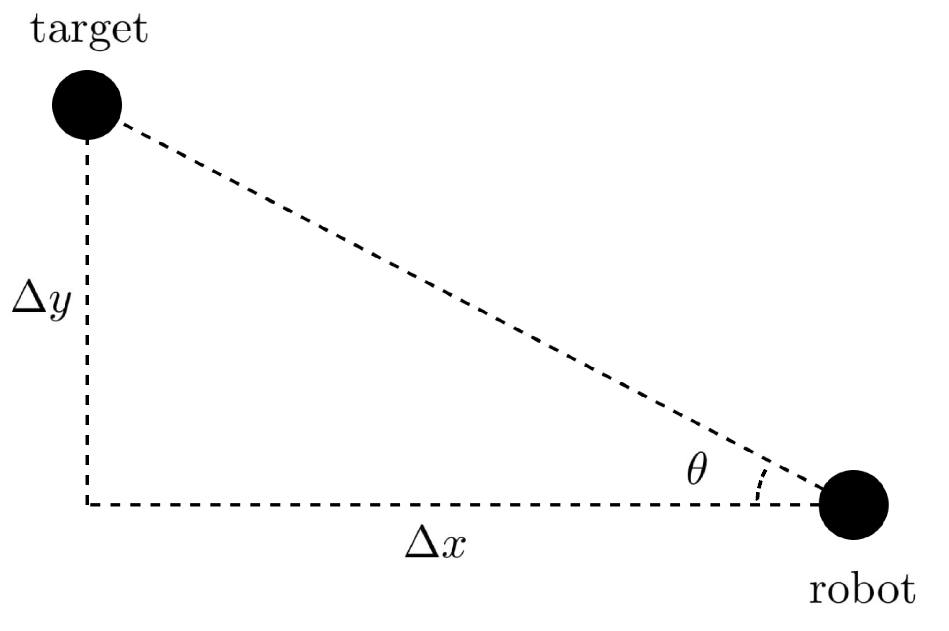
\includegraphics[width=\linewidth]{images/theta2.jpg}
\end{minipage}
\begin{minipage}{0.5\textwidth}\raggedleft
$$\quad \quad \quad \quad \theta = \pi - \left| \arctan\left(\frac{\Delta y}{\Delta x}\right) \right|$$ \\
\end{minipage}
\noindent
\\
The formula here takes $\pi$ and subtracts to it the angle between the robot and target because we want to take the full $180$ degrees minus the quantity show in the picture, which is $\theta$.
\\
\\
\textbf{$\Delta y < 0 \quad and \quad \Delta x < 0$}: \\ \\
\begin{minipage}{0.4\textwidth}
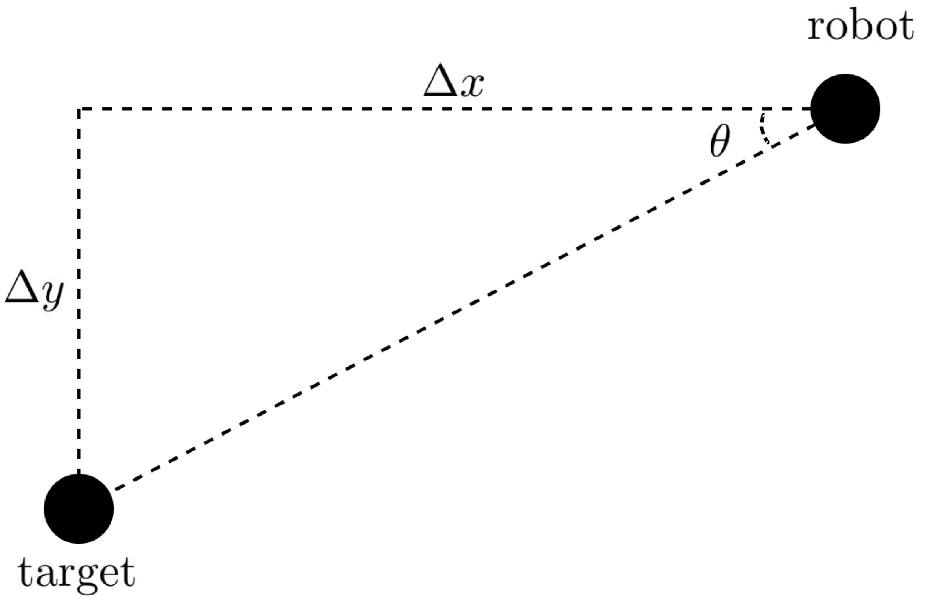
\includegraphics[width=\linewidth]{images/theta3.jpg}
\end{minipage}
\begin{minipage}{0.5\textwidth}\raggedleft
$$\quad \quad \quad \quad \theta = \frac{\pi}{2} -  \left| \arctan\left(\frac{\Delta x}{\Delta y}\right) \right|$$ \\
\end{minipage}
\noindent
\\
$\Delta x$ and $\Delta y$ get swapped because when moving upside down so do the opposite and adjacent sides.
\\
\\
\textbf{$\Delta y < 0 \quad and \quad \Delta x > 0$}: \\ \\
\begin{minipage}{0.4\textwidth}
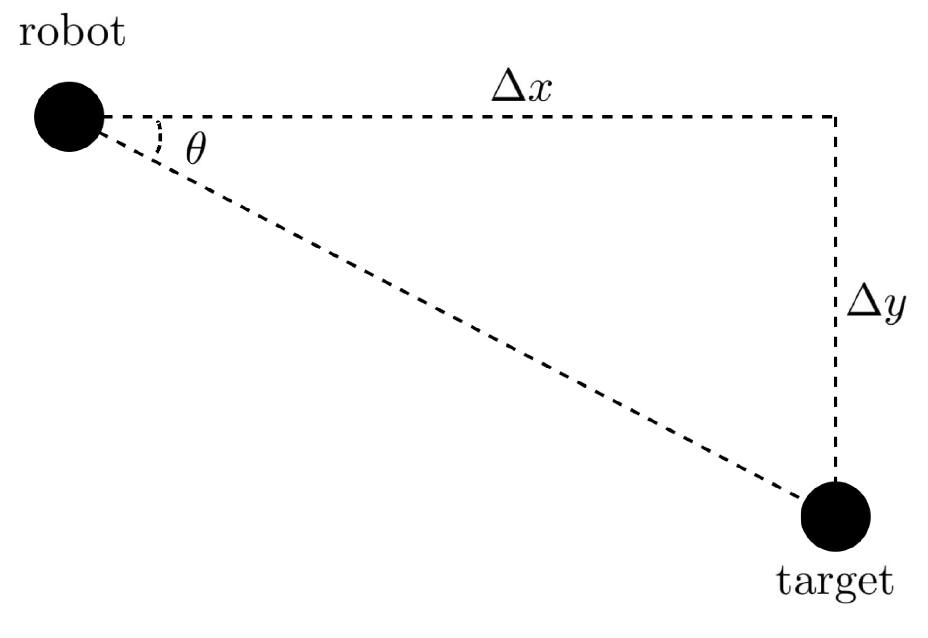
\includegraphics[width=\linewidth]{images/theta4.jpg}
\end{minipage}
\begin{minipage}{0.5\textwidth}\raggedleft
$$\quad \quad \quad \quad \theta = \frac{\pi}{2} + \left| \arctan\left(\frac{\Delta x}{\Delta y}\right) \right|$$ \\
\end{minipage}
\noindent
\\
The idea behind that $- \frac{\pi}{2}$ is that we want to take $90$ degrees plus the angle between the robot and the target. One quick look at the diagram will convince us of that. 
\par 
Now let us briefly explore the idea behind the \texttt{direction} function. The objective of this function is to decide whether to turn the robot left or right. As a reminder, by robot's orientation we mean the direction the robot is facing, while the target's angle is the angle which the robot should be orientated to in order to be headed towards the target. In a similar fashion to the \texttt{target\_theta} function, we split into four cases:
\begin{enumerate}
    \item Both the robot and \texttt{target\_theta} have a positive orientation. In this case we turn left if the robot's angle is smaller, right otherwise.
    \item Both are negative. Coincidentally the behavior in this case is the same as before.
    \item The robot's orientation is positive and the target's angle is negative. What we do here is calculate by how much we would have to move if we were to go both left and right. Right: we sum the angle of the robot and we subtract to it the angle of the target. Left: We take $\pi$ and remove the angle of the robot, then we add $\pi$ again and add the angle of the target. Only checking which one of this two quantities is bigger is left in order to decide where to go. The idea behind this case will be clearer when looking at the code.
    \item The robot's orientation is negative and the target's positive. We apply the same trick but we invert the decision we take. In other words if the first quantity is bigger than the second we turn left, right otherwise.
\end{enumerate}
As promised, here is the the algorithm which will hopefully clear things up.
\begin{lstlisting}[language=Python, caption=algorithm which decides whether to rotate RIGHT or LEFT]
def direction(robot, target): 
    #first and second case
    if robot.theta >= 0 and target.theta >= 0 or robot.theta <= 0 and target.theta <= 0:
        return LEFT if robot.theta < target.theta else RIGHT 
    
    #third case
    if robot.theta >= 0 and target.theta <= 0:
        right = robot.theta - target.theta
        left = 2 * math.pi - robot.theta + target.theta
        return RIGHT if right < left else LEFT

    #fourth case
    right = robot.theta - target.theta
    left = 2 * math.pi - robot.theta + target.theta
    return LEFT if right < left else RIGHT
\end{lstlisting}
\subsection{ROS2 communications}
The e\_puck robot is associated to the following ROS2 topics:
\begin{itemize}
    \item \textbf{\texttt{e\_puck/move}}: (subscriber). The message is an integer. It indicates the tile the robot should move to (to every tile a unique integer is assigned). It is the ROS2-BDI framework who publishes to this topic of course.
    \item \textbf{\texttt{e\_puck/position}}: (subscriber).The message contains four floats: the $x$, $y$, $z$ coordinates and the orientation $theta$. The supervisor publishes to this topic
    \item \textbf{\texttt{e\_puck/move\_completed}}: (publisher). The message is of empty type. It serves the purpose to indicate that the requested move was completed. Note that a service could have been used instead in this case.
\end{itemize}

\section{Supervisor} 
The supervisor is, at its core, a normal Webots robot. What makes it special is the ability to create and destroy new objects, access the parameters of other robots and objects (such as translation, orientation, scale, color, ecc...) and automatically subscribe to the simulation ROS2 topic \texttt{/clock}, which gives a very accurate estimation of how much time has elapsed since the beginning of the simulation.
\subsection{Purpose}
The purpose of the supervisor in this simulation is to:
\begin{itemize}
    \item Spawn new ducks every $n$ seconds and to remove the ducks whose internal clock has timed out. 
    \item Publish to the \texttt{e\_puck/position} topic the current position and orientation of the robot. Note that the e\_puck itself does not have access to its position, for this reason going through the supervisor to get this information is the only way to go. An alternative solution could have been to attach a GPS device to the robot, but to the author's mind it would have been a bit too convoluted of a solution. Besides, this would have implied not having access to the orientation, for the GPS does not provide that kind of information. 
    \item Publish to the \texttt{e\_puck/add\_belief} and \texttt{e\_puck/del\_belief} topics which indicate to the ROS2-BDI instance that a belief has to be added or deleted. This is necessary because ROS2-BDI needs to know where new ducks are spawned and if they get deleted.
\end{itemize}
\section{ROS2-BDI}
Let us walk through the general setup which would allow us to connect the Webots simulation to the ROS2-BDI instance correctly. Here is what needs to be done specifically: 
\begin{itemize}
    \item Setup the \textbf{initial beliefs}.
    \item Optionally, define an initial \textbf{desire set}.
    \item Optionally, designate the \textbf{reactive rules}.
    \item Create a \textbf{PDDL 2.1 domain}.
    \item Create the node definition for the \textbf{actions} specified in the domain definition.
    \item Optionally, describe the \textbf{sensors}, if any.
    \item Generate a \textbf{launcher} which will instantiate ROS2-BDI and the action/sensor nodes. 
\end{itemize}
What is going on, fundamentally, is that the framework will look at the domain and come up with a plan to satisfy the desires accordingly. The plan will be then executed thanks to the definitions of the actions. Furthermore the reactive rules, if defined, will be followed whenever necessary.
\subsection{PDDL domain}
Before all else we need to define the objects our world contains. These are the robot, the garbage, the box, the tile and the bin. Note that the tile represents a square in which objects can be positioned in the simulation. We can do exactly that by typing:  
\begin{lstlisting}[caption=PDDL 2.1 domain]
~;; Types ;;;;;;;;;;;;;;;;;;;;;;;;;;;;;;~
    (:@types@
        robot garbage box tile bin
    )~;; end Types ;;;;;;;;;;;;;;;;;;;;;;;;;~
\end{lstlisting}
Now the predicates (i.e. the statements about the world which can either be true or false):
\begin{lstlisting}[caption=Predicates definition]
(:@predicates@
    (at_rob ?r - robot ?t - tile)
    (at_gar ?g - garbage ?t - tile)
    (at_box ?b - box ?t - tile)
    (at_bin ?b - bin ?t - tile)
    (free ?r - robot)
    (adjacent ?t1 - tile ?t2 - tile)
    (walkable ?t - tile)
    (holding ?r - robot ?g - garbage)
    (deleted ?g - garbage)
    (to_recycle ?g - garbage)
)
\end{lstlisting}
Here is an explanation of the predicates:
\begin{itemize}
    \item \texttt{at\_x} indicates that the object of type \texttt{x} is located at tile $t$.
    \item \texttt{free} to say the robot is free and not holding anything.
    \item \texttt{adjacent} specifies that \texttt{t1} and \texttt{t2} are close to each other. This was done to lighten the work on the simulation side and let the ROS2-BDI program do the work. In fact if this condition was not there the move function would be orders of magnitude more complicated.
    \item \texttt{walkable} is used to mark tiles as either walkable or unwalkable. A tile cannot be crossed if an object or a box is on top of it.
    \item \texttt{holding} designates that the robot \texttt{r} is holding the piece of garbage \texttt{g}.
    \item When the supervisor deletes an object because it timed out the \texttt{deleted} predicate is set to true for that specific object.
    \item When an object has just been spawned, the \texttt{to\_recycle} predicate is initialized to true, which indicates that \texttt{g} needs to be collected and brought to the bin.
\end{itemize}
Only three actions are necessary to describe the simulation. These are \texttt{move}, \texttt{pickup} and \texttt{putdown}.
\begin{lstlisting}[caption=move action definition]
(:@durative-action@ move
    :@parameters@ (?r - robot ?from ?to - tile)
    :@duration@ (= ?duration 3)
    :@condition@ (and 
        (at start (at_rob ?r ?from))
        (over all (adjacent ?from ?to))
        (over all (walkable ?to))
    )
    :@effect@ (and
        (at start (not(at_rob ?r ?from)))
        (at end (at_rob ?r ?to))
    )
)
\end{lstlisting}
This action moves the robot from one tile to another. The preconditions require the robot to be at the starting tile in the beginning. What's more it is paramount the the destination tile is walkable and adjacent to the source tile. The effect is quite trivial: at the beginning the robot is not located at the source tile anymore and at the end it is situated at the destination one.
\begin{lstlisting}[caption=pickup action definiton]
(:@durative-action@ pickup
    :@parameters@ (?r - robot ?t - tile ?g - garbage)
    :@duration@ (= ?duration 1)
    :@condition@ (and
        (at start(free ?r))
        (at start (at_gar ?g ?t))
        (at start (at_rob ?r ?t))
    )
    :@effect@ (and
        (at end (not(free ?r)))
        (at end (not(at_gar ?g ?t)))
        (at end (holding ?r ?g))
    )
)
\end{lstlisting}
This action represent the moment where the robot picks up an object. For it to happen it is necessary that the robot and the object share the same position and for the robot to be free (i.e. not holding other objects). The effect is also self explanatory: the robot is not free anymore and is holding the object. The garbage is no longer positioned at its initial position.
\begin{lstlisting}[caption=Putdown action definition]
(:@durative-action@ putdown
    :@parameters@ (?r - robot ?t - tile ?b - bin ?g - garbage)
    :@duration@ (= ?duration 1)
    :@condition@ (and
        (over all (at_bin ?b ?t))
        (over all (at_rob ?r ?t))
        (at start (holding ?r ?g))
    )
    :@effect@ (and
        (at end(free ?r))
        (at end(at_gar ?g ?t))
        (at end (not(holding ?r ?g)))
    )
)
\end{lstlisting}
This action describes the act of the robot putting down an object. As a precondition it is obligatory that the robot holds the object and that the bin and the robot are located at the same tile. The effect is that the robot is now free and no longer holding on to anything. Furthermore the object is now at its destination.
\subsection{Belief set initialization}
To make sure that the ROS2-BDI instance behaves faithfully to the PDDL domain it is critical to initialize the set of predicates believed to be true at the beginning of the simulation. Additionally all the objects (robot, tile, box....) need to defined. All these beliefs need to be inserted into a \texttt{.yaml} file, respecting the syntax that will be shown.
\par
First things first, let us go over all the objects that need to be defined. 
\begin{itemize}
    \item The e\_puck robot.
    \item The bin
    \item All the boxes.
    \item All the $49$ tiles, named from \texttt{t0} to \texttt{t48}.
\end{itemize}
It is quite straightforward to write this kind of declaration inside the \texttt{.yaml} file. For example if we wanted to declare the e\_puck robot we would write:
\begin{lstlisting}
- @name@: "e_puck"
  @pddl_type@: 1
  @type@: "robot"
\end{lstlisting}
A \texttt{pddl\_type = 1} indicates that we are discussing an object declaration, while a \texttt{pddl\_type = 2} means we are working with a predicate.
\par
Now, onto the predicates initialization:
\begin{itemize}
    \item The position of the robot, the bin and the boxes.
    \item The robot must be initialized as free by setting the \texttt{free} predicate to \texttt{true}.
    \item Each tile which does not contain a box or any other object needs to be declared as \texttt{walkable}.
    \item For each tile all of its adjacencies ought to be itemized. For simplicity's sake only the up, down, right and left directions were considered, while the diagonals were not taken notice of. This can be done by making use of the \texttt{adjacent} predicate.
\end{itemize}
Once again, the syntax for this kind of statement is trivial. Say we wanted to show that the tile \texttt{t1} and \texttt{t3} are adjacent. To do that the following piece of code would be sufficient.
\begin{lstlisting}
- @name@: "adjacent"
  @pddl_type@: 2
  @params@: 
    - "t1"
    - "t3"
- @name@: "adjacent"
  @pddl_type@: 2
  @params@: 
    - "t3"
    - "t1"
\end{lstlisting}
It is needed to declare both \texttt{t1} adjacent to \texttt{t3} and vice versa because the planner may be checking the predicate from either side.
\subsection{Reactive rules}
Reactive rules allow us to dynamically modify the belief and desire sets via some predefined rules. They are optional but a very nice to have feature and essential for some scenarios. The first scenario does not actually need reactive rules, however, the second scenario, in which ducks appear as well as disappear, finds them vital. Consequently let us go through them. We only need two of them: One that pushes the desire to retrieve objects whenever they appear and one to delete the desire to retrieve the objects that have timed out. Like belief and desire set initialization, they are defined inside a \texttt{.yaml} file.
\begin{lstlisting}[caption=Reactive rule that pushes the desire to retrieve an object as soon as it spawns]
- @condition@:
    @clauses@:
    - @literals@:
        - @check@: "EX"
            @condition_to_check@:
            @name@: "{x}"
            @pddl_type@: 1
            @type@: "garbage"
      
        - @check@: "T"
            @condition_to_check@:
            @name@: "to_recycle"
            @pddl_type@: 2
            @params@:
                - "{x}"
      
        - @check@: "F"
            @condition_to_check@:
            @name@: "deleted"
            @pddl_type@: 2
            @params@:
                - "{x}"

@reactive_rules@: 
    - @set@: desire
    @operation@: ADD
    @value@:
        @name@: "recycle_{x}"
        @priority@: 0.6
        @deadline@: 1000
        @value@:
        - @name@: "at_gar"
          @pddl_type@: 2
          @params@:
            - "{x}"
            - "t1"
\end{lstlisting}
Basically if the first three checks are verified at any point in time the reactive rule condition is set off. The first condition checks whether an object of type garbage exists; the second whether it needs to be recycled or not and the third makes sure it has not been deleted already. If all three conditions are satisfied the desire to retrieve the object and put it next to the bin is pushed. Now, Let us look at the second reactive rule.
\begin{lstlisting}[caption=Reactive rule that deletes the desire to retrieve an object if it no longer exists]
- @condition@:  
    @clauses@:
      - @literals@:
        - @check@: "T"
          @condition_to_check@:
            @name@: "deleted"
            @pddl_type@: 2
            @params@:
              - "{x}"

  @reactive_rules@:
    - @set@: desire
      @operation@: DEL
      @value@:
        @name@: "recycle_{x}" 
        @priority@: 0.6
        @deadline@: 1000
        @value@:
          - @name@: "at_gar"
            @pddl_type@: 2
            @params@:
              - "{x}"
              - "t1"    
\end{lstlisting}
If the \texttt{deleted} predicate is true for the object \texttt{\{x\}} then the reactive rule's execution is triggered. As a result of that the desire to recycle that object is removed from the \texttt{belief\_set}.
\subsection{Actions}
One action is defined for each durative action inside the PDDL domain, that means move, pickup and put down. The definition is embedded inside a ROS2 node, which is especially convenient as it allows the use of ROS2 functionalities inside of it. Basically the idea is to use ROS2 communication tools to contact the simulation and tell it what to do. The advantageous thing of this is that everything will take care of itself automatically as the action execution is triggered autonomously by the ROS2-BDI instance. In other words if the planner believes that the best course of action in a certain time step of the simulation is to perform a move action, ROS2 topics and services will be called from inside the action node definition and will tell the robot to move to the designated tile.
\par
Let us look at the definition of one of these actions, the move action.
\begin{lstlisting} [language=c++, caption=Move action node]
class Move : public BDIActionExecutor {
public:
    Move() : BDIActionExecutor("move", 1) {
        publisher_ = this->create_publisher<std_msgs::msg::Int16>("move", 10);

        subscriber_ = this->create_subscription<std_msgs::msg::Empty>(
            "move_completed", 4,
            std::bind(&Move::move_completed_callback, this, _1));

        publisher_->on_activate(); // activate publisher on node creation
    }

    float advanceWork() {
        publisher_->publish(create_msg());

        if (move_completed) {
            move_completed = false;
            return 1.0f;
        }

        return 0.025f;
    }

    void move_completed_callback(const std_msgs::msg::Empty::SharedPtr msg) {
        move_completed = true;
    }

    std_msgs::msg::Int16 create_msg() {
        std::vector<std::string> arguments = this->getArguments();

        auto msg = std_msgs::msg::Int16();
        msg.data = arguments[2][1] - '0'; // -'0' trick to convert char to int
        if (arguments[2][2] >= '0' && arguments[2][2] <= '9')
            msg.data = (arguments[2][1] - '0') * 10 + (arguments[2][2] - '0');
        
        return msg;
    }
};
\end{lstlisting}
In the constructor the node is instantiating the publisher for the \texttt{/move} topic. This node will be told from ROS2-BDI when to activate and when it happens it will publish to the \texttt{/move} topic. It also subscribes to the \texttt{/move\_completed} topic in case the e\_puck terminates its movement earlier than anticipated. 
\par
The constructor's parameter \texttt{"move"} is used this node to the right action. The parameter \texttt{1} is used to decide how many times a second the method \texttt{advanceWork()} is called.
\par
The method \texttt{advanceWork()}, which in this case is called $1$ time per second, is used as the feedback of the action by returning a float. The action will be considered uncompleted until the cumulative return values of the \texttt{advanceWork()} will be less than $1$. The function is defined in a similar fashion to a state machine: it keeps returning \texttt{0.025f}, but if the flag \texttt{completed} is true (which happens if a message arrives from the \texttt{move\_completed} topic) it returns \texttt{1.0f}. The value \texttt{0.25f} was set because the move action is believed to last at most $40$ seconds, therefore either the action concludes naturally at the end of this time period or it interrupts earlier due to the flag being set to \texttt{true}.
\par
The method \texttt{advanceWork()} main job is to publish to the topic \texttt{e\_puck/move}, which it does at the line number $14$. The message could be sent up to $40$ times but it will not be an issue since the extra messages will by no means impede the e\_puck's calculations. The message contains the tile towards which the robot should move. It is calculated thanks to the API call \texttt{getArguments()} which contains the name of the action and its parameters.
\subsection{Launcher} In the ROS2-BDI architecture the launcher's main job is to instantiate the core node's and make the necessary connections to the actions automatically. In addition to that it allows the user to define some key parameters such as the planning configuration (online or offline), the reschedule policy, the beliefs \texttt{.yaml} file, the reactive rules \texttt{.yaml} file and other less interesting parameters for this particular simulation. The aforementioned parameters were the main ones played with across each different scenario. 
\subsection{Overall architecture} 
As promised at the beginning of this chapter, here is the overall architecture for this simulation:
\begin{figure}[H]
\centering
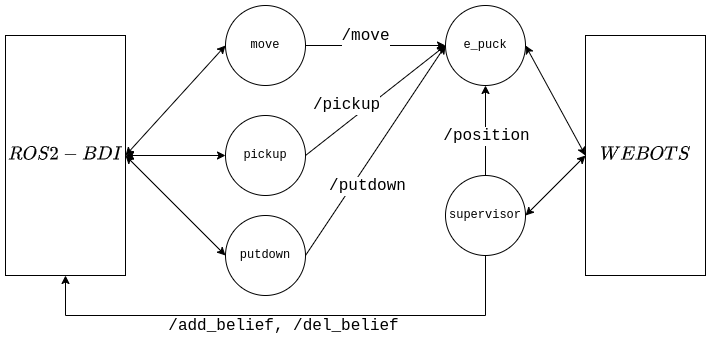
\includegraphics[width=\textwidth]{images/simulation_architecture.png}
\caption{The simulation's architecture}
\end{figure}
The two big rectangles are the representation of the ROS2-BDI instance and the Webots instance. The circles are ROS2 nodes and they communicate with each other using ROS2 communications. Unidirectional arrows represent ROS2 topics, while bidirectional arrows are either ROS2 services or actions. 
\par
The three nodes \texttt{move}, \texttt{pickup} and \texttt{putdown} are automatically generated by ROS2-BDI when launching and exchanged messages are handled autonomously by the ROS2-BDI architecture. They instruct the robot e\_puck robot when to perform those actions with the depicted topics.
\par 
The e\_puck node reads the messages from the action topics and leverages the Webots API which are implemented upon ROS2 to tell the graphical simulation to perform the requested action. The name of these ROS2 communications are omitted, for they are hidden to the programmer since Webots API's handle everything on the background. They are however indicated in the diagram unnamed. A clarification is needed here, the messages are used just to turn instruct the graphical interface to turn the motors, not to indicate an abstract action such as \texttt{move t2}.
\par
The supervisor gets the information about the world from the Webots instance thank to the provided API's implemented on top of ROS2. It publishes to the topic \texttt{/position} which indicates the position of the robot. Furthermore it publishes to the topics \texttt{add\_belief} and \texttt{del\_belief} whenever a new objects appears and disappears. It is the supervisor's job to handle the belief set for this kind of action because it is also responsible of spawning and deleting new objects.
\newpage

      \chapter{Experimental results}
The objective of this validation is dual: on one hand it tries to show that the framework can be used and works as expected in a more solid simulator. Some attempts at this have already been made by the designers of the framework, however, an ad hoc environment which may not always agree with the conditions of a real world scenario was used. Contrariwise, Webots is a highly regarded 3D graphic robot simulator which should be satisfactory in this regard.
\par
On the other hand the objective was to show the better performance of the online approach in comparison to the offline planner in highly dynamic environments. This analysis has already been carried out by the developers of the ROS2-BDI architecture, therefore this extra analysis only serves as a way of strengthening that idea with some additional scenarios and different parameters.

\section{Additional scenarios description}
As a reminder, here are the four scenario tested;
\begin{enumerate}
    \item the basic situation consists in a $7$ by $7$ grid where objects appear in random positions and a robot tries to pick them up as effectively as possible and bring them to the bin.
    \item Same as above with the addition of a new timer for each new object. If it goes off the object disappears and is no longer retrievable.
    \item Same as above, furthermore a new robot whose task is uncorrelated to the e\_puck and moves around the map, sometimes blocking the path.
    \item As previously, what's more the possibility to pick up as many objects as the robots wants. For all other simulations the robot could only carry up to one object at a time.
\end{enumerate}

\section{Results}
Each configuration was run $30$ times, the result metrics are the average measures. Here is a quick explanation of the parameters:
\begin{itemize}
    \item \textbf{\texttt{SPAWN\_RATE}} is the time, in seconds, that passes between the apparition of each object.
    \item \textbf{\texttt{LIFE\_SPAN}} is the timer, in seconds, after which the object disappears.
    \item \textbf{\texttt{DUCK\_COUNT}} is the total amount of objects spawned during the simulation.
    \item \textbf{\texttt{PLANNER}} indicates which planner (online/offline) was used.
    \item \textbf{\texttt{miss\_rate}} is the rate of objects failed to retrieve in percentage. 
    \item \textbf{\texttt{avg\_retrieve\_time}} is the average time, in seconds, the robot spent retrieving objects, from the moment they spawn to the moment they are brought to the bin.
\end{itemize}
Here are the results of the validation process for the scenario number $1$:
\begin{center}
\begin{tabular}{|c|c|c|c|c|c|}
    \hline
     \multicolumn{4}{|c|}{\textbf{Parameters}} & \multicolumn{2}{|c|}{\textbf{Results}} \\
     \hline
     \textbf{\texttt{SPAWN\_RATE}} & \textbf{\texttt{LIFE\_SPAN}} & \textbf{\texttt{DUCK\_COUNT}} & \textbf{\texttt{PLANNER}} & \textbf{\texttt{miss\_rate}} & \textbf{\texttt{avg\_retrieve\_time}} \\
     \hline
     foo & bar & foo & bar & foo & bar \\
     bar & foo & bar & foo & bar & foo \\
     foo & bar & foo & bar & foo & bar \\
     bar & foo & bar & foo & bar & foo \\
     foo & bar & foo & bar & foo & bar \\
     \hline
\end{tabular}
\end{center}

Here are the results of the validation process for the scenario number $2$:
\begin{center}
\begin{tabular}{|c|c|c|c|c|c|}
    \hline
     \multicolumn{4}{|c|}{\textbf{Parameters}} & \multicolumn{2}{|c|}{\textbf{Results}} \\
     \hline
     \textbf{\texttt{SPAWN\_RATE}} & \textbf{\texttt{LIFE\_SPAN}} & \textbf{\texttt{DUCK\_COUNT}} & \textbf{\texttt{PLANNER}} & \textbf{\texttt{miss\_rate}} & \textbf{\texttt{avg\_retrieve\_time}} \\
     \hline
     foo & bar & foo & bar & foo & bar \\
     bar & foo & bar & foo & bar & foo \\
     foo & bar & foo & bar & foo & bar \\
     bar & foo & bar & foo & bar & foo \\
     foo & bar & foo & bar & foo & bar \\
     \hline
\end{tabular}
\end{center}

Here are the results of the validation process for the scenario number $3$:
\begin{center}
\begin{tabular}{|c|c|c|c|c|c|}
    \hline
     \multicolumn{4}{|c|}{\textbf{Parameters}} & \multicolumn{2}{|c|}{\textbf{Results}} \\
     \hline
     \textbf{\texttt{SPAWN\_RATE}} & \textbf{\texttt{LIFE\_SPAN}} & \textbf{\texttt{DUCK\_COUNT}} & \textbf{\texttt{PLANNER}} & \textbf{\texttt{miss\_rate}} & \textbf{\texttt{avg\_retrieve\_time}} \\
     \hline
     foo & bar & foo & bar & foo & bar \\
     bar & foo & bar & foo & bar & foo \\
     foo & bar & foo & bar & foo & bar \\
     bar & foo & bar & foo & bar & foo \\
     foo & bar & foo & bar & foo & bar \\
     \hline
\end{tabular}
\end{center}

Here are the results of the validation process for the scenario number $4$:
\begin{center}
\begin{tabular}{|c|c|c|c|c|c|}
    \hline
     \multicolumn{4}{|c|}{\textbf{Parameters}} & \multicolumn{2}{|c|}{\textbf{Results}} \\
     \hline
     \textbf{\texttt{SPAWN\_RATE}} & \textbf{\texttt{LIFE\_SPAN}} & \textbf{\texttt{DUCK\_COUNT}} & \textbf{\texttt{PLANNER}} & \textbf{\texttt{miss\_rate}} & \textbf{\texttt{avg\_retrieve\_time}} \\
     \hline
     foo & bar & foo & bar & foo & bar \\
     bar & foo & bar & foo & bar & foo \\
     foo & bar & foo & bar & foo & bar \\
     bar & foo & bar & foo & bar & foo \\
     foo & bar & foo & bar & foo & bar \\
     \hline
\end{tabular}
\end{center}

\section{Remarks on the results}
TODO

\newpage
      \chapter{Flexibility evaluation} 
The goal of this chapter is to show that once the initial set up is done, it is easy to adapt ROS2-BDI to virtually any new scenario. To be more specific, we will check whether the application follows well the principle of scalability and modularity by presenting some practical examples.
\par 
It is important to mention that the last two additions are to be considered speculative as they were not actually implemented, for the author decided to focus their time on different aspects of the project. However the speculation will, in all probability, be faithful to a possible real implementation. 
\par
As a reminder, the most basic situation consists in a $7$ by $7$ grid where objects appear in random positions and a robot tries to pick them up as effectively as possible and bring them to the bin. Now we shall look at the modifications needed to change the scenario, focusing mostly only on the ROS2-BDI architecture.

\section{Adding a timer}
Let us suppose that for whatever reason we must pick objects up before a timer runs out and we have already implemented the basic scenario. Here are the adjustments needed.

\subsection{Reactive rule addition} Basically the only change needed on the ROS2-BDI side. We need to add a reactive rule that deletes the desire to retrieve an object if it were to be deleted. The implementation is shown in Listing 3.11 in chapter 3. This rule is triggered if the predicate \texttt{deleted} which is removed from the belief set by the supervisor using the \texttt{/del\_belief} topic.
\par
This hopefully gives an idea of the level of modularity of ROS2-BDI since all we had to do to adapt was adding another tiny module (the reactive rule) to our scenario. Although the change is minimal, the way the planner will operate will be drastically different. That is because in case the objects disappear often the number of plan abortions will increase significantly. The great thing about this though is that in spite of the growth in complexity of the plans, the work the programmer has to carry out is not far from the same, for ROS2-BDI will take care of every additional complication.

\section{Adding an uncorrelated agent}
On top of the timer a new agent moves around the map, sometimes blocking the planned path by the e\_puck.

\subsection{Belief set management}
The modifications here are simpler in comparison to the previous alteration. We have already defined a \texttt{walkable} predicate which we can use to infer that the tile the extra robot is currently occupying cannot be accessed. The belief addition and deletion is taken care of by the supervisor, which, using the \texttt{/add\_belief} and \texttt{/del\_belief} topics, tells ROS2-BDI that when a tile becomes accessible/inaccessible.

\section{Multiple objects collection}
Now we are going to see how to allow the robot to pick up as many objects as it wants.

\subsection{PDDL domain alteration} 
If we take a look a the \texttt{pickup} action we can see that among its preconditions there is a predicate \texttt{(at start (free ?r))} which means that the robot must be free before the action begins. If we want to allow the robot to pick up as many objects as it wants we could just remove this predicate from the set of precondition.
\par
If instead we want the robot to hold at most $n$ objects we could try using functions instead. This could be done by adding a function \texttt{(capacity ?r - robot)}. After this all that is left is to:
\begin{itemize}
    \item Initialize the new function to any value we want in the belief set.
    \item Add the precondition \texttt{(at start (> capacity ?r) 0)} to the \texttt{pickup} action.
    \item Add the effect \texttt{(at end (decrease (capacity ?r) 1))} to the \texttt{pickup} action.
    \item Add the effect \texttt{(at end (increase (capacity ?r) 1))} to the \texttt{putdown} action.
\end{itemize}
Once again the complexity of the new solution is very low and the impact on the planner is of great importance. This is testament to the modularity of the architecture which allows for radical changes in the internal behavior of the system with very little effort.

\section{Simulation layout modification} 
Let us now suppose that the layout of the physical simulation changes, i.e. the map gets bigger or some objects (like robot, box or bin) change position. Obviously the simulation definition needs to change. The changes on ROS2-BDI are more interesting though.
\par
Whatever the change is the only thing that needs to be altered is the belief set initialization. For example if we want to make the map bigger we would just need to define more tiles, set them to \texttt{walkable} and instantiate adjacencies accordingly. If we wish to change the position of the robot, the bin or anything else, we just need to change the parameters of the \texttt{at} predicate by modifying the referenced tile.
\par
This effortless modification when upsizing the simulation's dimensions is a clear indication that the ROS2-BDI architecture is incontrovertibly scalar when it comes to this kind of remodeling.

\section{Adding multiple agents}
Since ROS2-BDI is a MAS (Multi agent system) it only makes sense that we look into the differences in set up when two or more agents populate the simulation. Ideally we would want the agents to cooperate, meaning that it should never happen that different robots try to retrieve the same object, for it would be a waste of time.
There are countless ways to do achieve that, the following solution is just one of many possible implementations.
\par
Two new predicates \texttt{(is\_being\_retrieved ?g - garbage ?r - robot)} and \texttt{(booked ?g - garbage ?r - robot)} are added, the first specifies whether an agent has committed to pick that particular object up while the second one is its complement. Furthermore, a new action with duration equal to zero is added. Its goal is to manage the aforementioned predicates. Here is the implementation:
\begin{lstlisting}
    (:@durative-action@ book_garbage
        :@parameters@ (?r - robot ?g - garbage)
        :@duration@ (= ?duration 0)
        :@condition@ (and 
            (at start (is_not_being_retrieved ?g ?r))
        )
        :@effect@ (and 
            (at end (not (is_not_being_retrieved ?g ?r)))
            (at end (booked ?g ?r)
        )
    )
\end{lstlisting}
The reason behind the decision to use two complementary predicates is that PDDL 2.1 support for negative preconditions is poor for the time being.
To complement this new addition we need to make sure that a plan is not outputted if an agent has not booked a piece of garbage. We can accomplish that by adding an auxiliary precondition to the \texttt{pickup} action. That is \texttt{(over all (booked ?g ?r))}.
The reason behind the duration being equal to zero is that it is hoped the planner will put the action at the beginning of the plan, thus booking the piece of garbage immediately and disallowing other agents to reserve that object.
\par
More agents means more ROS2 nodes, therefore we need to include an additional one in the launcher of the project, which, as usual, will take care of the interconnections on its own.
\par
This expansion is by all means the most convoluted of all the extensions. However, it also greatly increases the proportion of the project. In light of this analysis we can conclude that ROS2-BDI is also quite easily scalable, seeing that it allows for the inclusion of multiple agent with a reasonably low level of effort.
\newpage
      \chapter{Conclusion} 
TODO



\newpage
      
      
    \endgroup


    % bibliography - bibtex format
    %
    % add chapter to index
    \addcontentsline{toc}{chapter}{Bibliography}
    % alphabetical order of authors
    \bibliographystyle{plain}
    \bibliography{biblio}
%%%%%%%%%%%%%%%%%%%%%%%%%%%%%%%%%%%%%%%%%%%%%%%%%%%%%%%%%%%%%%%%%%%%%%%%%%
%%%%%%%%%%%%%%%%%%%%%%%%%%%%%%%%%%%%%%%%%%%%%%%%%%%%%%%%%%%%%%%%%%%%%%%%%%
%% Nota
%%%%%%%%%%%%%%%%%%%%%%%%%%%%%%%%%%%%%%%%%%%%%%%%%%%%%%%%%%%%%%%%%%%%%%%%%%
%% In the bibliography, all the sources consulted for the dissertation 
%% have to be cited and listed in alphabetical order by the 
%% first author's surname.
%%
%% According to the source material, the quotation has to be as follows:
%%
%% BOOKS
%% Surname and initial/s of the name/s of the author/s, date of edition,
%% publishing house and (if applicable) number of edition.
%% 
%% JOURNAL ARTICLES 
%% Surname and initial/s of the first name/s of the author/s,
%% title of the article, name of the journal, volume number, issue number
%% and page numbers.
%% 
%% CONFERENCE PAPERS
%% Surname and initial/s of the name/s of the author/s,
%% year of the conference, title of the article, name of the conference,
%% place of the conference, conference dates, page numbers.
%% 
%% CITING WEB RESOURCES
%% The consulted webpages have to be listed in alphabetical order. 
%% It is necessary to:
%%   - Copy the specific URL (the web address) of the consulted webpage
%%   - If available, indicate the surname and first name of the author/s,
%%     the title and subtitle of the text
%%   - If available, indicate the last date you retrieved the webpage
%%     (day/month/year).   
%%%%%%%%%%%%%%%%%%%%%%%%%%%%%%%%%%%%%%%%%%%%%%%%%%%%%%%%%%%%%%%%%%%%%%%%%%
%%%%%%%%%%%%%%%%%%%%%%%%%%%%%%%%%%%%%%%%%%%%%%%%%%%%%%%%%%%%%%%%%%%%%%%%%%
    

    %\titleformat{\chapter}
        %{\normalfont\Huge\bfseries}{Appendix \thechapter}{1em}{}
    % Appendix / attachment section - optional
    %\appendix
    %\chapter{Title first appendix}

Lorem ipsum dolor sit amet, consectetur adipiscing elit. Donec sed nunc orci. Aliquam nec nisl vitae sapien pulvinar dictum quis non urna. Suspendisse at dui a erat aliquam vestibulum. Quisque ultrices pellentesque pellentesque. Pellentesque egestas quam sed blandit tempus. Sed congue nec risus posuere euismod. Maecenas ut lacus id mauris sagittis egestas a eu dui. Class aptent taciti sociosqu ad litora torquent per conubia nostra, per inceptos himenaeos. Pellentesque at ultrices tellus. Ut eu purus eget sem iaculis ultricies sed non lorem. Curabitur gravida dui eget ex vestibulum venenatis. Phasellus gravida tellus velit, non eleifend justo lobortis eget. 

\section{Title}
Lorem ipsum dolor sit amet, consectetur adipiscing elit. Donec sed nunc orci. Aliquam nec nisl vitae sapien pulvinar dictum quis non urna. Suspendisse at dui a erat aliquam vestibulum. Quisque ultrices pellentesque pellentesque. Pellentesque egestas quam sed blandit tempus. Sed congue nec risus posuere euismod. Maecenas ut lacus id mauris sagittis egestas a eu dui. Class aptent taciti sociosqu ad litora torquent per conubia nostra, per inceptos himenaeos. Pellentesque at ultrices tellus. Ut eu purus eget sem iaculis ultricies sed non lorem. Curabitur gravida dui eget ex vestibulum venenatis. Phasellus gravida tellus velit, non eleifend justo lobortis eget. 

\subsection{Sub-title}
Lorem ipsum dolor sit amet, consectetur adipiscing elit. Donec sed nunc orci. Aliquam nec nisl vitae sapien pulvinar dictum quis non urna. Suspendisse at dui a erat aliquam vestibulum. Quisque ultrices pellentesque pellentesque. Pellentesque egestas quam sed blandit tempus. Sed congue nec risus posuere euismod. Maecenas ut lacus id mauris sagittis egestas a eu dui. Class aptent taciti sociosqu ad litora torquent per conubia nostra, per inceptos himenaeos. Pellentesque at ultrices tellus. Ut eu purus eget sem iaculis ultricies sed non lorem. Curabitur gravida dui eget ex vestibulum venenatis. Phasellus gravida tellus velit, non eleifend justo lobortis eget. 


\chapter{Title first appendix}

Lorem ipsum dolor sit amet, consectetur adipiscing elit. Donec sed nunc orci. Aliquam nec nisl vitae sapien pulvinar dictum quis non urna. Suspendisse at dui a erat aliquam vestibulum. Quisque ultrices pellentesque pellentesque. Pellentesque egestas quam sed blandit tempus. Sed congue nec risus posuere euismod. Maecenas ut lacus id mauris sagittis egestas a eu dui. Class aptent taciti sociosqu ad litora torquent per conubia nostra, per inceptos himenaeos. Pellentesque at ultrices tellus. Ut eu purus eget sem iaculis ultricies sed non lorem. Curabitur gravida dui eget ex vestibulum venenatis. Phasellus gravida tellus velit, non eleifend justo lobortis eget. 

\section{Title}
Lorem ipsum dolor sit amet, consectetur adipiscing elit. Donec sed nunc orci. Aliquam nec nisl vitae sapien pulvinar dictum quis non urna. Suspendisse at dui a erat aliquam vestibulum. Quisque ultrices pellentesque pellentesque. Pellentesque egestas quam sed blandit tempus. Sed congue nec risus posuere euismod. Maecenas ut lacus id mauris sagittis egestas a eu dui. Class aptent taciti sociosqu ad litora torquent per conubia nostra, per inceptos himenaeos. Pellentesque at ultrices tellus. Ut eu purus eget sem iaculis ultricies sed non lorem. Curabitur gravida dui eget ex vestibulum venenatis. Phasellus gravida tellus velit, non eleifend justo lobortis eget. 

\subsection{Sub-title}
Lorem ipsum dolor sit amet, consectetur adipiscing elit. Donec sed nunc orci. Aliquam nec nisl vitae sapien pulvinar dictum quis non urna. Suspendisse at dui a erat aliquam vestibulum. Quisque ultrices pellentesque pellentesque. Pellentesque egestas quam sed blandit tempus. Sed congue nec risus posuere euismod. Maecenas ut lacus id mauris sagittis egestas a eu dui. Class aptent taciti sociosqu ad litora torquent per conubia nostra, per inceptos himenaeos. Pellentesque at ultrices tellus. Ut eu purus eget sem iaculis ultricies sed non lorem. Curabitur gravida dui eget ex vestibulum venenatis. Phasellus gravida tellus velit, non eleifend justo lobortis eget. 




\end{document}
